\section{Análisis de Diseño del Cohete}

El diseño aerodinámico y estructural del vehículo PDA STARS se desarrolló mediante un proceso iterativo de modelado CAD tridimensional en Autodesk Fusion 360 y simulación aerodinámica en OpenRocket (archivo oficial \texttt{211\_PDASTARS\_Diseño.ork}), buscando satisfacer simultáneamente el requerimiento de apogeo a 300 m y la estabilidad pasiva $\ge 2,0\text{ cal}$.

\begin{figure}[H]
\centering
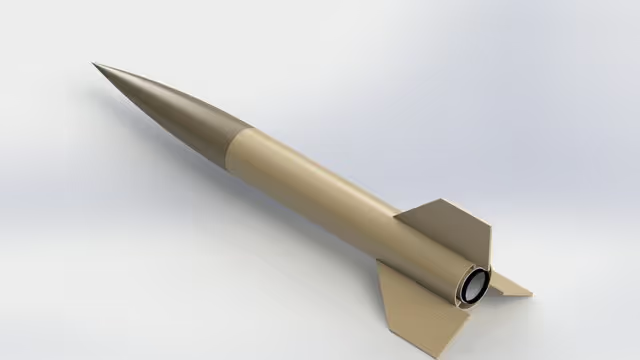
\includegraphics[width=0.75\linewidth]{cad_cohete.png}
\caption{Modelo digital tridimensional (CAD) del cohete PDA STARS en Fusion 360.}
\label{fig:cad_cohete}
\end{figure}

\subsection{Arquitectura Modular del Vehículo}
El cohete presenta una longitud total de \textbf{68,5 cm} (685 mm) y un diámetro exterior de \textbf{66,0 mm} (tubo Kraft comercial BT-80 con espesor de pared de 0,8 mm), dividido en tres módulos estructurales:
\begin{enumerate}[leftmargin=1.5em]
    \item \textbf{Ojiva Haack (Von Kármán):} Longitud de \textbf{13,0 cm}, fabricada mediante impresión FDM en filamento PETG sólido (masa de 39,7 g). Su perfil continuo optimiza la transición de presión en régimen subsónico compresible.
    \item \textbf{Bahía de Carga Útil y Aviónica:} Longitud de \textbf{19,0 cm} en tubo Kraft BT-80 (masa de 60,0 g). Aloja el contenedor impreso en 3D con el microcontrolador Seeeduino XIAO, sensores barométricos/inerciales, batería NiMH, altímetro digital y cáncamo estructural de retención.
    \item \textbf{Fuselaje Principal y Propulsión:} Longitud de \textbf{36,5 cm} en tubo Kraft BT-80 (masa de 30,0 g). Alberga el sistema de recuperación (paracaídas de 40 cm y manta Nomex de 15x15 cm), tubo portamotor concéntrico de 29 mm y 14,0 cm de longitud, dos anillos de centrado en PETG-CF y retén inferior roscado.
    \item \textbf{Conjunto de Aletas Estructurales:} Tres aletas de forma libre con perfil biconvexo sustentador (airfoil), envergadura de 12,0 cm, cuerda de raíz de 14,5 cm, cuerda de punta de 2,0 cm y espesor de 2,0 mm en PETG reforzado con fibra de carbono (PETG-CF, masa total del conjunto de 64,0 g), fijadas a través del fuselaje hasta el portamotor con resina epoxi de grado aeronáutico.
\end{enumerate}

\begin{figure}[H]
\centering
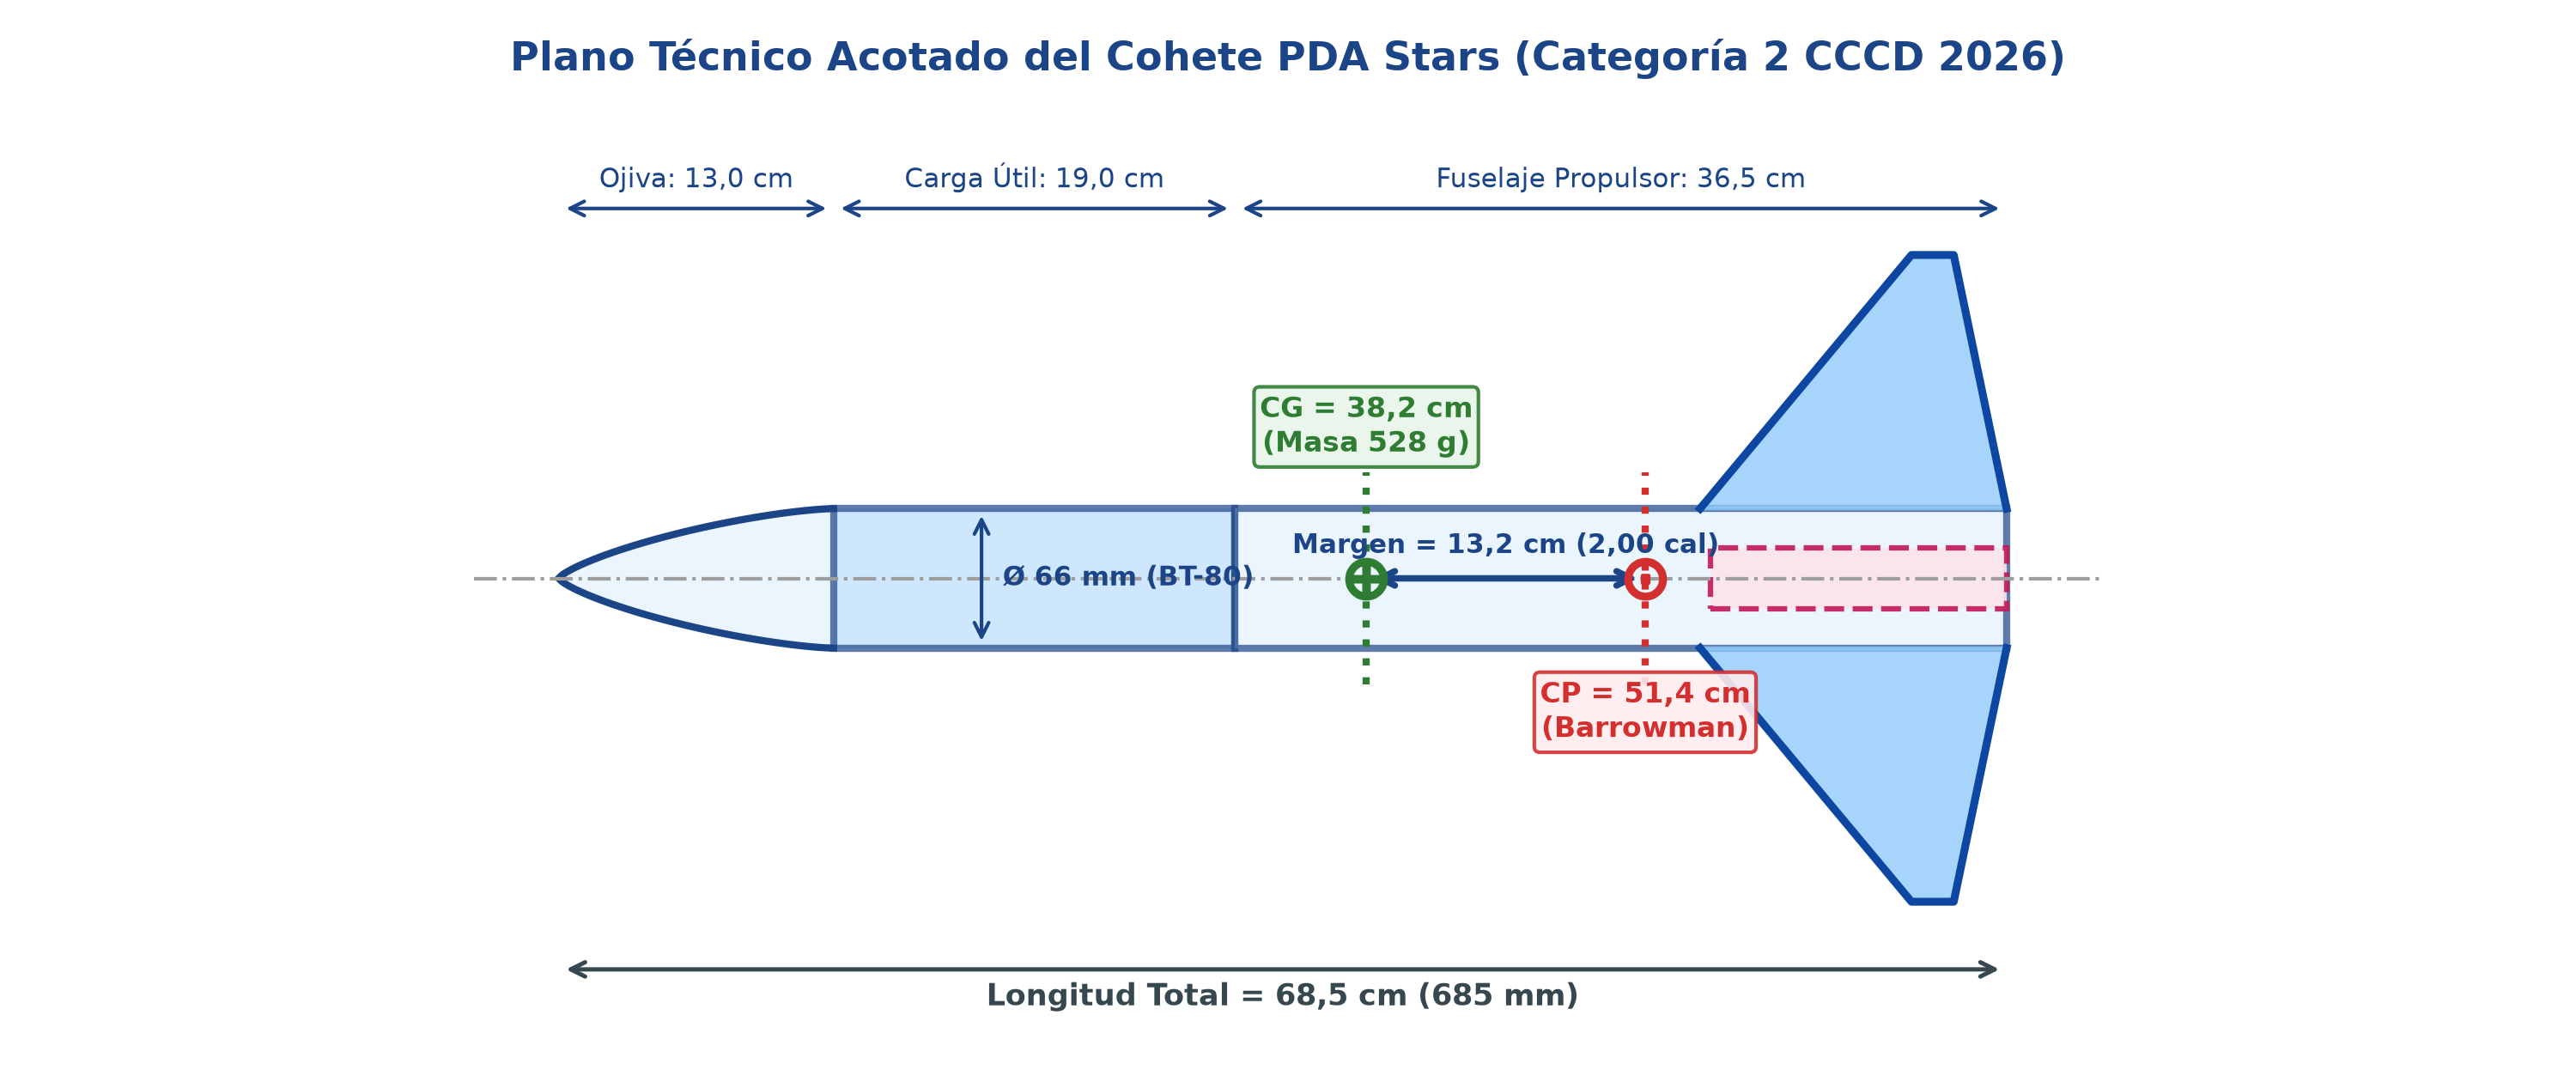
\includegraphics[width=0.95\linewidth]{fig_plano_acotado_cohete.png}
\caption{Plano técnico acotado y dimensionamiento estructural del cohete PDA STARS.}
\label{fig:plano_acotado}
\end{figure}

\begin{figure}[H]
\centering
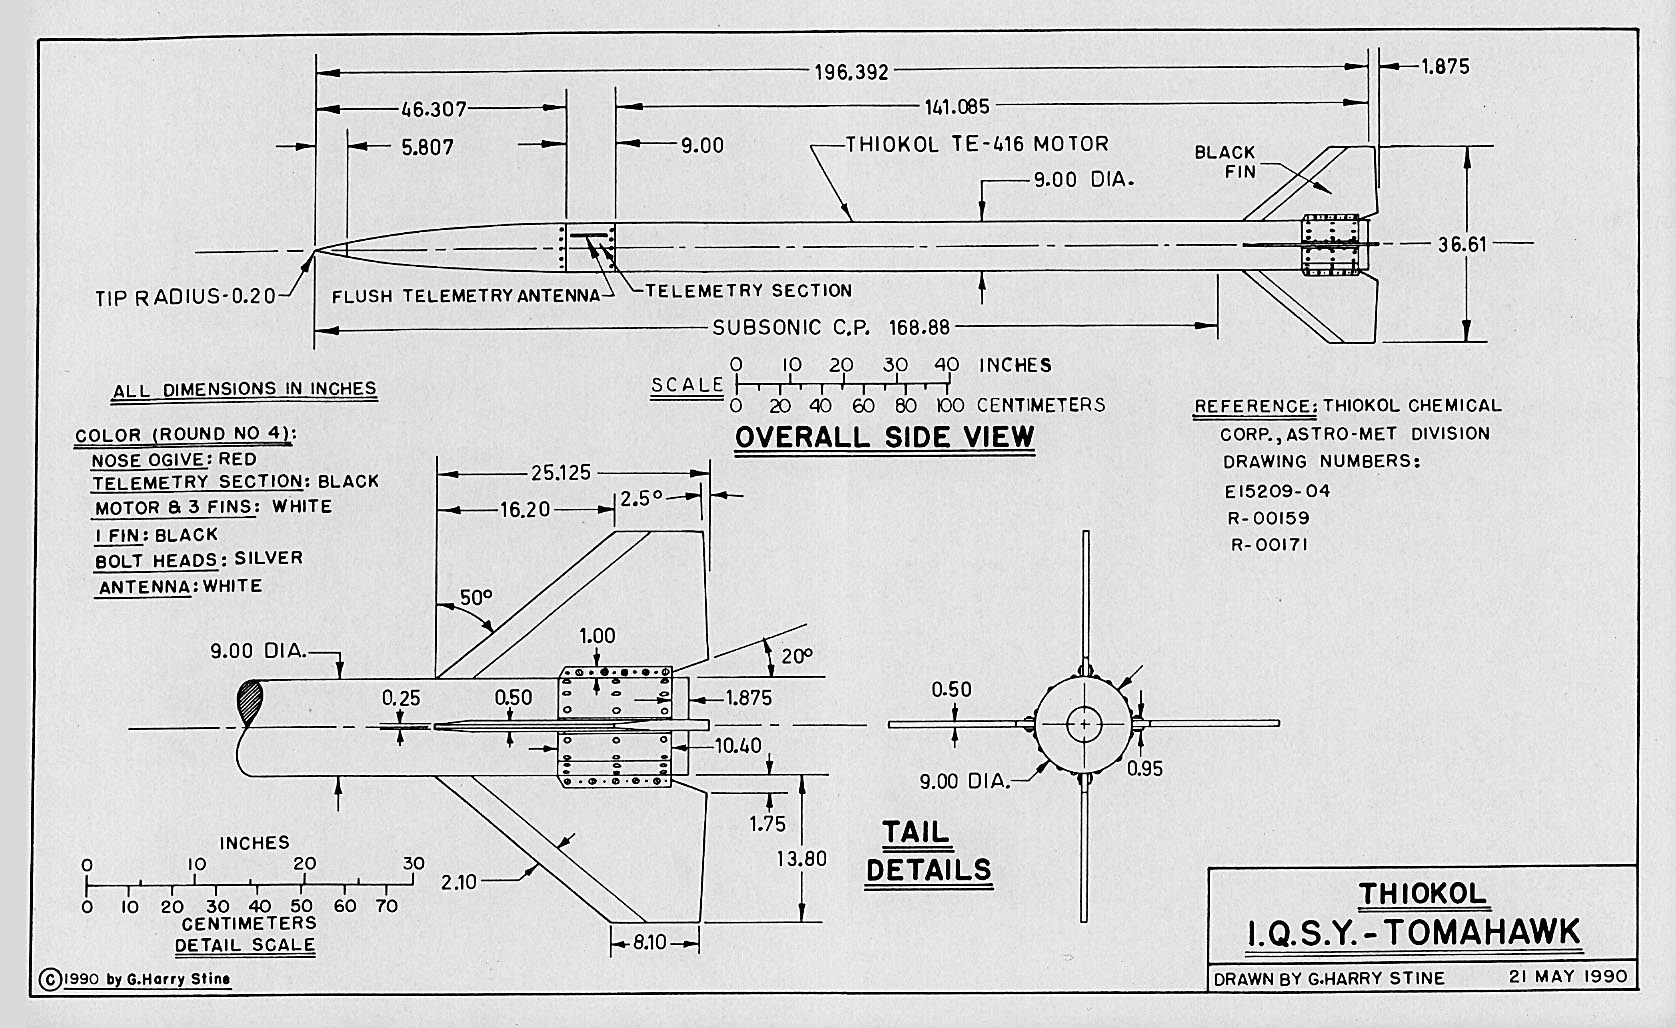
\includegraphics[width=0.85\linewidth]{plano_cohete.png}
\caption{Plano de conjunto y ensamble en software de diseño mecánico.}
\label{fig:plano_mecanico}
\end{figure}

\subsection{Distribución de Masas y Margen Estático de Estabilidad}
En la configuración definitiva de vuelo, el Centro de Gravedad real ($CG$) se ubica a \textbf{38,2 cm} desde el vértice de la ojiva con el vehículo totalmente cargado en rampa (masa total de 528 g). El Centro de Presión teórico ($CP$), calculado en OpenRocket mediante las formulaciones aerodinámicas clásicas de Barrowman, se sitúa a \textbf{51,4 cm}.

La separación estática resultante es de:
\begin{equation}
    \Delta x = CP - CG = 51,4\text{ cm} - 38,2\text{ cm} = 13,2\text{ cm}
\end{equation}
Expresado en función del calibre de referencia ($D = 6,6\text{ cm}$):
\begin{equation}
    \text{Margen Estático} = \frac{CP - CG}{D} = \frac{13,2\text{ cm}}{6,6\text{ cm}} = \mathbf{2,00\text{ calibres}}
\end{equation}
Durante la fase propulsada, a medida que el grano del motor Estes F15 se consume (60 g de propelente quemado), el $CG$ se desplaza ligeramente hacia adelante hasta los 37,8 cm, incrementando el margen estático a \textbf{2,05 calibres} en el momento del agotamiento (\textit{burnout}), lo cual garantiza un vuelo estrictamente estable en todas las etapas.
